\documentclass[12pt, twopage]{article}
\linespread{1.25}

\usepackage[utf8]{inputenc}
\usepackage{amsthm}
\usepackage{amsmath}

\usepackage{amsfonts}
\usepackage[slovak]{babel}
\usepackage{graphicx}
\usepackage[hidelinks, breaklinks]{hyperref}

\theoremstyle{definition}
\newtheorem{example}{Príklad}
\newtheorem{definition}{Definícia}

%[]

%\begin{definition}[]
%	Obsah...
%\end{definition}

\title{\textbf{Planimetria - geometria v rovine}}
\date{\today}
\author{\textit{Educat - vzdelávacie centrum}}

\newcommand{\blank}
{\underline{\hspace{4cm}}}

\newcommand{\overarrow}[1]
{\overset{\longleftrightarrow}{#1}}



\begin{document}
	\maketitle
	
	\section{Základy planimetrie}
	
	Z tabuľky doplň pojmy k definíciám.
	\begin{center}
		\begin{tabular}{|ccc|}
			\hline
			bod & priamka & polpriamka \\
			úsečka & rovina & polrovina \\
			stred úsečky & krajné body úsečky& \\
			\hline
		\end{tabular}
	\end{center}
	
	\begin{enumerate}
		\item \blank označujeme veľkými tlačenými písmenami. Zobrazujeme ním pozíciu v rovine alebo priestore.
		
		\item \blank je nekonečne dlhá rovná čiara, ktorá prechádza 2 bodmi. Označujeme ju malými písmenami so znakom rovnej čiary nad ňou, napr. $\overarrow{p}$, alebo podobne 2 bodmi, ktorými prechádza, napr. $\overarrow{AB}$.
		
		\item \blank je časť priamky $\overarrow{AB}$, ktorá je oddelená bodom $P$, ktorý na nej leží. Tento bod ju rozeľuje na 2 navzájom opačné \blank $\overrightarrow{AP}$ a $\overrightarrow{PA}$.
		
		\item \blank je prienik 2 navzájom opačných polpriamok $\overrightarrow{AB}$ a $\overrightarrow{BA}$. Body $A$ a $B$ nazývame \blank. Jej dĺžku značíme $|AB|$. Bod $S$, ktorý na nej leží a pre ktorý platí $|AS| = |SB|$ sa nazýva \blank.
		
		\item \blank označujeme malými gréckymi písmenami, napr. $\sigma$, alebo inými spôsobmi, podľa toho, ako je určená:
		\begin{itemize}
			\item 3 bodmi, ktoré neležia na jednej priamke - značíme $\overarrow{ABC}$
			\item priamkou a bodom, ktorý na nej neleží - značíme $\overarrow{pM}$
			\item 2 rôznymi priamkami - značíme $\overarrow{pq}$
		\end{itemize}
		
		\item \blank je časť roviny oddelená priamkou. Ak $\overarrow{p} \in \sigma$. Ak máme daný bod $M$ mimo tejto priamky, tak ju značíme $\overrightarrow{pM}$. Alebo ak je priamka $p$ daná bodmi $A$ a $B$, tak ju značíme $\overrightarrow{ABM}$ 
		
		
	\end{enumerate}
	
	Z tabuľky doplň správne zápisy daným popisom.
	
	\begin{center}
		\begin{tabular}{|ccc|}
			\hline
			$P \in \overline{p}$ & $\overline{p} \in \sigma$ & $P \notin \overline{p}$ \\
			$\overline{p} \notin \sigma$ & $A \in \sigma$ & $A \notin \sigma$\\
			\hline
		\end{tabular}
	\end{center}
	
	\begin{center}
		\begin{tabular}{|c|c|}
			\hline 
			Popis & Zápis \\
			\hline
			bod $P$ leží na priamke $p$ & \hspace{3cm} \\
			\hline
			bod $P$ nelží na priamke $p$ & \\
			\hline
			priamka $p$ leží v rovine $\sigma$ & \\
			\hline
			priamka $p$ neleží v rovine $\sigma$ & \\
			\hline
			bod $A$ leží v rovine $\sigma$ & \\
			\hline
			bod $A$ neleží v rovine $\sigma$ & \\
			\hline
			
		\end{tabular}
	\end{center}
	
	\newpage
	\section{Uhly}
	
	Do definície uhlu doplň pojmy z tabuľky.
	
	\begin{center}
		\begin{tabular}{|ccc|}
			\hline
			uhol & vrchol & ramená \\
			polpriamky & & \\
			\hline
		\end{tabular}
	\end{center}
	
	\begin{definition}[Uhol]
		\blank je časť roviny určená dvoma \blank so spoločným začiatkom.
		Tento začiatok sa nazýva \blank a dané \blank voláme jeho \blank. Uhol $AVB$ značíme $\angle AVB$ resp. $\angle \alpha$ alebo iné malé grécke písmeno. Jeho veľkosť značíme $|\angle AVB|$ resp. $|\angle \alpha|$.
	\end{definition}
	
	\subsection{Delenie uhlov podľa veľkosti}
	
	Z tabuľky doplň do rozhodovacieho stromu typy uhlov podľa podmienok na ich veľkosť.
	
	\begin{center}
		\begin{tabular}{|ccc|}
			\hline
			ostrý & pravý & konvexný \\
			tupý & nekonvexný/konkávny & nulový \\
			priamy & & \\
			\hline
		\end{tabular}
	\end{center} 
	
	\begin{center}
		 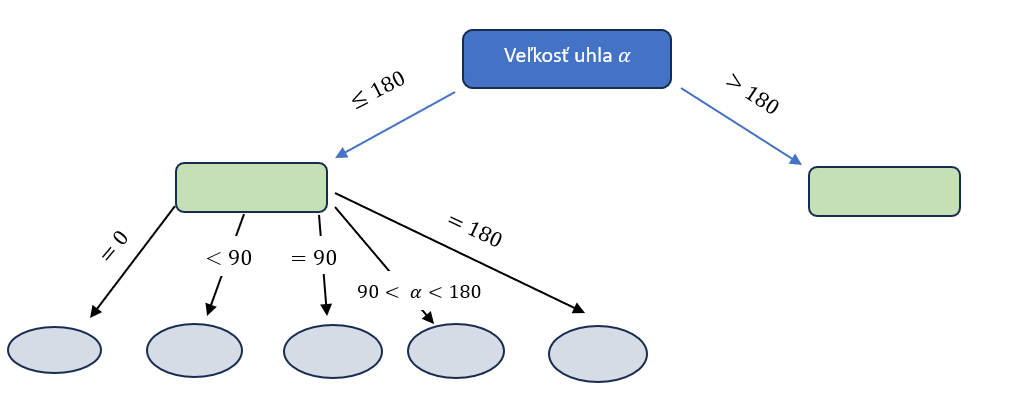
\includegraphics[width=\linewidth]{assets/uhly_strom.png}
	\end{center}
	
	Na nasledovnej dvojici uhlov vyznač, ktorý z nich konvexný a ktorý konkávny. 
	
	\begin{center}
		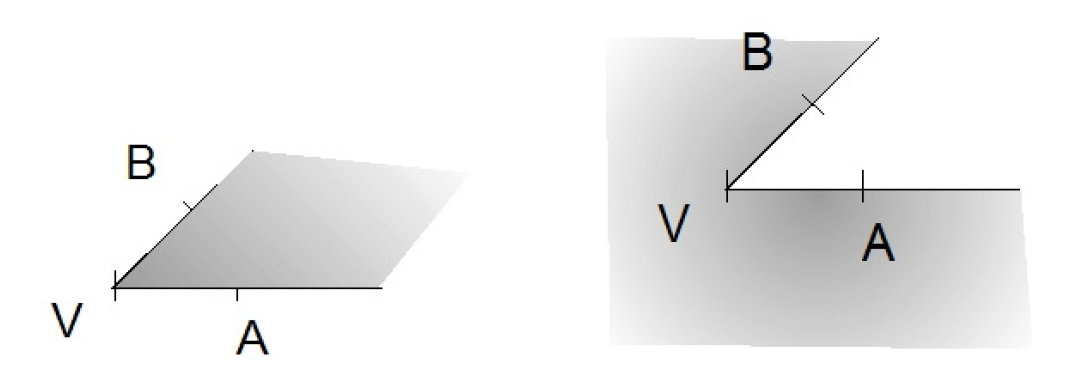
\includegraphics[width=\linewidth]{assets/von_vnu_uhol.png}
	\end{center}
	
	Zrejme ak $\angle AVB$ je konvexný uhol, tak spolu s konkávnym uhlom $\angle BVA$ dávajú 360 stupňov.
	
	\subsection{Delenie dvojíc uhlov podľa susednosti}
	
	K nasledujúcim dvojiciam uhlov napíš, kde sú zobrazené susedné, striedavé, súhlasné a vrcholové uhly.\\
	
	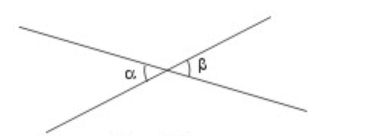
\includegraphics{assets/vrcholove_uhly.png}
	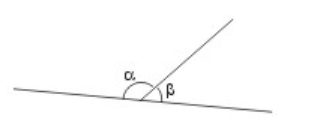
\includegraphics{assets/susedne_uhly.png}\\
	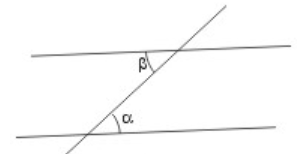
\includegraphics{assets/striedave_uhly.png}
	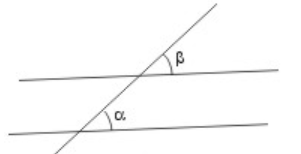
\includegraphics{assets/suhlasne_uhly.png}
	
	Pre niektoré dvojice platí, že dokopy dávajú 180 stupňov alebo sú rovnaké. Pre ktorú dvojicu platí ktoré tvrdenie?
	
	\newpage
	
	\section{Rovinné útvary}
	
	\subsection{Štvorec}
	
	\subsection{Obdĺžnik}
	
	\subsection{Kosodĺžnik}
	
	\subsection{Kosoštvorec}
	
	\subsection{Lichobežník}
	
	\subsection{Mnohouholník}
\end{document}